\section{Results and Discussion}
System-level simulation was performed with representative AI inference workloads.

\begin{itemize}
  \item \textbf{Standby Power}: $>$30\% reduction by migrating cold data to FeRAM-backed tier.
  \item \textbf{Resume Latency}: reduced to $\mu$s–ms range, enabling instant resume across power cycles.
  \item \textbf{Endurance}: $10^{12}$ writes/year fits within FeRAM capability for checkpoint traffic.
\end{itemize}

% ===== Fig.2: Access vs retention (clear colored markers) =====
\begin{figure}[!t]
\centering
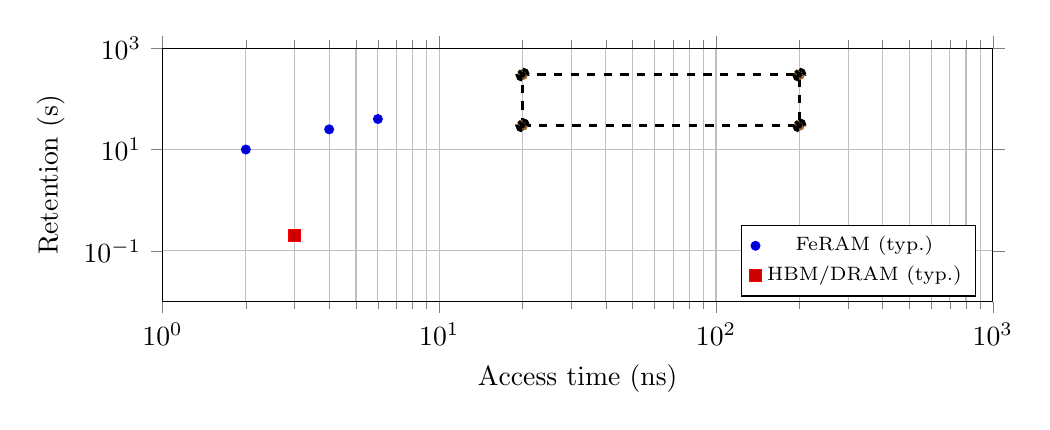
\begin{tikzpicture}
\begin{axis}[
  width=\linewidth, height=4.8cm,
  xmode=log, ymode=log,
  xmin=1e0, xmax=1e3, ymin=1e-2, ymax=1e3,
  xlabel={Access time (ns)}, ylabel={Retention (s)},
  grid=both, tick align=outside, clip=false,
  legend style={font=\scriptsize, at={(0.98,0.02)}, anchor=south east}
]

% --- FeRAM (blue circles) ---
\addplot+[only marks, mark=*, mark size=1.6pt, blue]
  coordinates {(2,10) (4,25) (6,40)};
\addlegendentry{FeRAM (typ.)}

% --- HBM/DRAM (red squares) ---
\addplot+[only marks, mark=square*, mark size=2.2pt, red]
  coordinates {(3,0.2)};
\addlegendentry{HBM/DRAM (typ.)}

% --- Optional "target window" (dashed box). DELETE this block if not wanted. ---
\addplot+[black, dashed, very thick]
  coordinates {(20,30) (200,30) (200,300) (20,300) (20,30)};

\end{axis}
\end{tikzpicture}
\caption{Access time vs.\ retention. **Red square: HBM**, **blue circles: FeRAM**. The dashed box indicates a \emph{future co-design target window} where fast \& persistent operation overlap. Remove the dashed box by deleting the last \texttt{\textbackslash addplot} block.}
\label{fig:retention_access}
\end{figure}
